\chapter{Background}\label{chp:background}


\section{Passwords}
Passwords are the common way of authenticating users upon access to sites on the Internet, the idea is that only the user and the target service knows the password, and the user have to provide the correct password before access are granted. Passwords are a much discussed theme and claiming that passwords are usually not used in the correct manner is not an overreaction. The main problem seems to be the fact that good passwords and the human memory does not go well together. For passwords to be sufficient as authentication each user has to be forced into using long complex password, or even use one generated for them, with the problem being that it is easily forgotten. Further more, if a user was able to memorize \emph{one} "good" password, he will probably use this for all of his accounts, so that if one of the services is compromised and user information leaked, all his accounts may be compromised. With all of this in mind it is easy to say that everybody should use complex, unique passwords for each account, but in practice this is not feasible. Florêncio and Herley ~\cite{password-habits} conducted a large scale study of passwords habits in 2007, revealing that a user on average has 25 different accounts protected by passwords. On average these sites are protected by about 7 distinct password, where 5 of them are rapidly re-used.
\par Password authentication requires the authenticating server to store something related to the password, if this is stolen the password will in most cases be compromised as well, even if the server did not store the clear text password, attackers will, in most cases, be able to retrieve the password eventually. After obtaining the username and password for one service the attacker would try this user data on other services and compromise these as well. 
\par If a user was to have different passwords for each site, these might still easily be compromised. Ives et al. ~\cite{domino-effect} discuss this "domino effect", where intrusion to one domain can compromise several others, if users have re-used passwords.  A normal user will typically try to log in by trial-and-error ~\cite{single-pw-auth}, if the first password does not work, the user will try with another of his passwords. This way may passwords might be lost through phising attacks where a user is tricked into trying to log in to a fake site. It is thus clear that some kind of system is needed to allow a human user to manage strong passwords. The best case would be if each user, for each of his 25 accounts had a unique password of satisfying strength, this is of course not possible.

\subsection{Password strength}\label{password-strength}
How to measure the strength of passwords is a well known and discussed problem, but the general idea is that password strength is related to how strong a password is against brute force attacks. Length and complexity is the most thought of parameters to measure such strength. A perfect password would thus be one as long as allowed by the system consisting of random characters from all possible characters, this one would also be changed frequently. All these characteristics despite how the human brain works. Yan et al.~\cite{memorability_yan} investigate the trade of between security of passwords versus memorability allowing humans to remember them. An important regarding this trade-off is that most sites applying advices and policies on how to create strong passwords, does not take into account if the advices passwords are hard or easy to remember. Point being that there is no point in having a strong password if the user is going to forget it. They suggest that passwords should appear random but be constructed using a  mnemonic structure such ass passphrases. The idea here is to generate a random looking password by memorizing a familiar sentence and using the first letters of each word as the password. Florêncio et al.~\cite{strong-pws_florencio} investigate another matter; do strong passwords accomplish anything? The point being that no matter how long and complex password users chose they are still subject to the most dangerous and common threats (phising, keylogging or access attacks), as discussed in the previous section. The reason for enforcing strong passwords seems to be to protect against bulk guessing attacks, against other attacks, typically offline attacks, shorter passwords is usually sufficient. 
\paragraph{Password strength meters} are a common way used by many sites on the Internet to aid their users when selecting passwords

The conclusion on what "good" passwords are, is not clear, but the one thing agreed upon seems to be that re-use of passwords are the biggest threat. It is a fact that the human brain is not capable of remembering different passwords for each account on the Internet, thus the need for an aiding application such as the one discussed in this project. 



Miller \cite{magic-seven_miller} showed that the human brain cannot store more than $7\pm 2$ chunks of information in immediate memory.
\subsection{Attacks}
Passwords are often the only barrier stopping adversaries from directly accessing the accounts of a user. The combination of user name and password are the easiest point of entry to access, and thus the first logical point of attack. There are several methods used to attack password authentication, trying to retrieve passwords. The most important attacks and their respective mitigation technique \cite{nist-guide, strong-pws_florencio}, will be discussed in the following section. 
\paragraph{Capturing} of passwords directly from the server responsible for the authentication involves the attack acquiring password data through breaking into the data storage, eavesdropping on communication channels or through monitoring the user by other means. The first most basic threat are to simply steal the stored password from an insecure server, this would require a weak configured server storing the passwords in plain text. This is mitigated mostly by only storing only cryptographic hashes of passwords. The hashes allows the server to authenticate users while preventing attackers from determining the actual passwords without \emph{cracking} the hashes. This approach would require the attackers to go through several steps. First acquiring the hash of a user account or a whole file of hashes for a site, next one would try to find a sequence of string yielding the same hash as the actual password. How hard it is to crack a hash depends on the strength of the password and can be mitigated by choosing strong passwords and changing these frequently.\emph{ Rainbow tables }~\cite{rainbow-tables} are a technique employed by attackers to speed up this process. Rainbow tables are precomputed table of hashes, allows the attacker to compute a set of hashes once and use these values several times, thus providing a space-time trade-off. This involves using more space, since all the computed hash values would have to be stored somewhere, but allowing a much shorter computation time to brute-force a hash. The technique stores chains of hashes as shown in figure ~\ref{rainbow-table}, storing only the first and last value of the chain. The attacker then search for a given hash in the set of end points, if no match are found the hash function is applied and a new search conducted. This process continues, until a match is found, the plain text is then then computed from the start value of the chain, applying the hash function the same amount of times it took to find a match in the chain. \todo{rewrite - more precise }

\begin{figure}[h]
    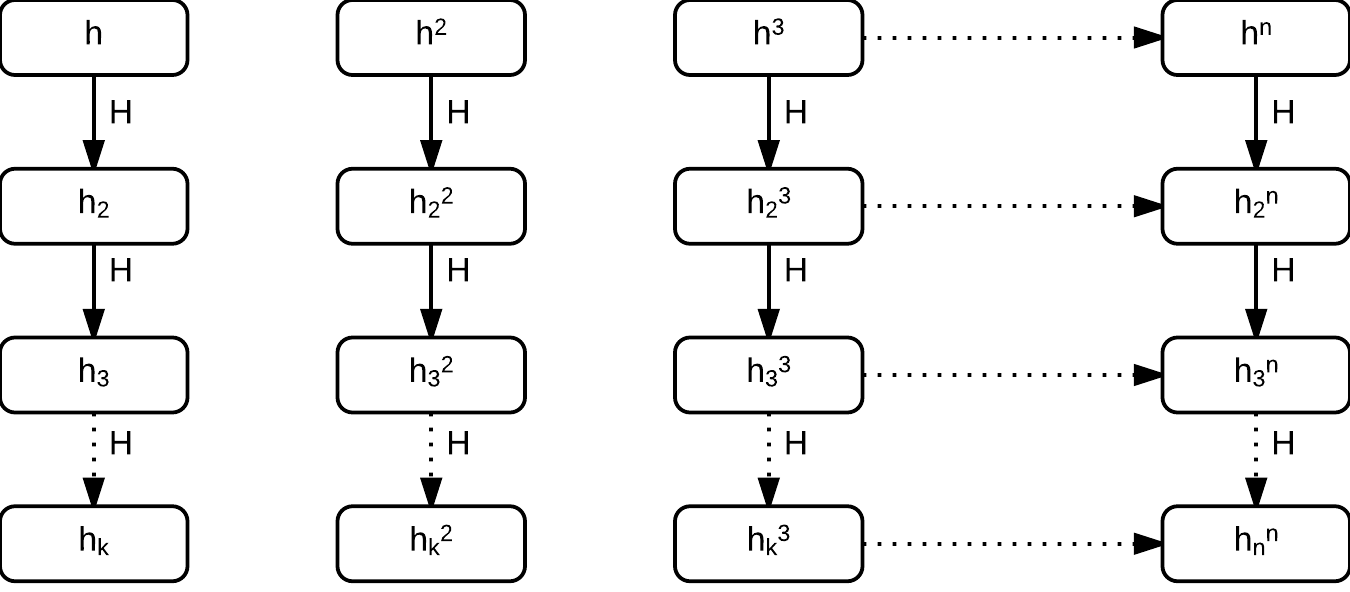
\includegraphics[width=\textwidth]{rainbow-table}
    \caption{Rainbow table}
    \label{rainbow-table}
\end{figure}

\subsection{Password Storage}

\subsection{Alternative authentication methods}

\section{Human Behavior}
"Good passwords" as discussed in \ref{password-strength} does not go well with the human memory. The first limitation which will be an important property later are the limitation to how much data we can store in immediate memory, this limit was showed to be 7 chunks of data at once~\cite{magic-seven_miller}. This data can not be from a random selection which is what a good password requires.   

\section{Password Management}

\section{Usability and Security Challenges}

\section{Browser Extensions}
Modern computer users shift towards doing more and more work through their web browsers. Web applications have become popular due to the ubiquity of browsers, thus allowing web apps to run anywhere. A web app can run at any platform running a web browser, allowing the application to run on multiple platforms as well as different devices. Updates can be applied quickly without having to distribute patches to a possibly huge amount of devices.
\par Browser extensions add additional features to the web browser allowing the user to tweak the experience of the web. Typical examples are extensions adding to or tweaking already present features of the browser such as changing how bookmarks are managed, or adding additional features such as blocking advertisements. Lately browser extensions has been extended even further allowing standalone applications to be developed running as native applications ~\cite{chrome-app-blog}. This allows developers to create desktop apps using the same technology as in web apps, mainly HMTL5, Javascript and CCS.
\par Browser extensions introduce some security concerns which must not be forgotten while developing applications using this environment. Chrome extensions run in the browser with access to both the DOM of the active page as well as the native file system and connected devices. The overall architecture of the application is summarized in \autoref{extension-architecture}


\begin{figure}[h]
    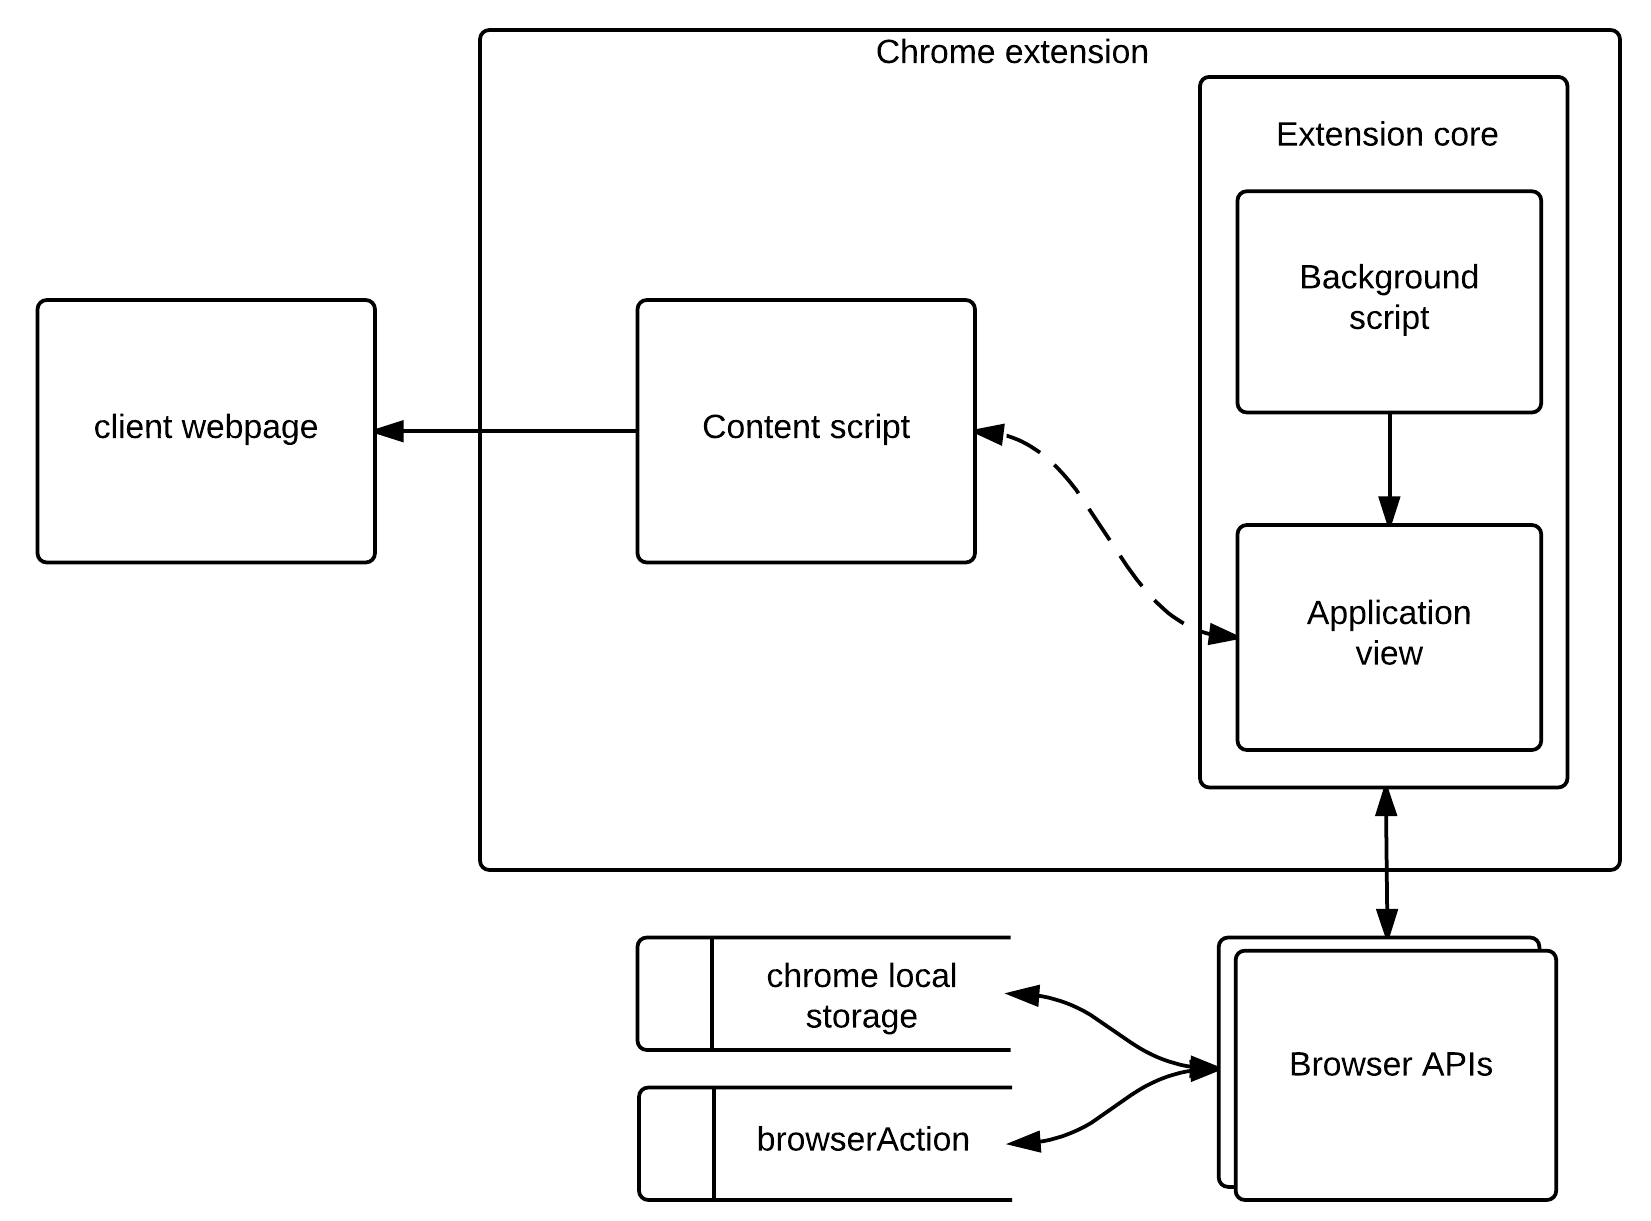
\includegraphics[width=\textwidth]{chrome-extension-architecture}
    \caption{Chrome extension architecture}
    \label{extension-architecture}
\end{figure}
\par This project will utilize chrome extensions to create a password manager running in the users browser.
\section{Usability Model}

\section{Security Model}




